\section*{Dati e risultati}

\subsection*{Raddrizzatore di precisione a semionda}

\begin{wrapfloat}{figure}{O}{0pt}
        \def\svgwidth{0.4\textwidth}
        \subimport{figure/}{raddrizzatore.pdf_tex}
        \caption{Raddrizzatore di precisione a semionda. Alimentato, inizialmente con una $V\ped{in}\,=\,\SI{1.02}{\volt}$ di frequenza $\nu\,=\,\SI{50}{\hertz}$.}
        \label{fig:radd}
\end{wrapfloat}

Lo scopo di questo raddrizzatore di precisione a semionda è lo stesso di quello di un normale raddrizzatore di tensione asemionda. Tuttavia vi è una caratteristica sostanzialmente differente tra le due tiplogie di raddrizzatori di tensione. Nel caso di un raddrizzatore normale, quindi di un circuito che sfrutta solo le peculiarità di un diodo, vi è una differenza di potenziale ai capi del diodo (normalmente, se il diodo è al silicio, questa ddp. vale $\SI{0.6}{\volt}$). Questa differenza di potenziale si riperquote sul segnale in uscita ($V\ped{out}$), che pur seguendo fedelmente il segnale in ingresso ($V\ped{in}$) risulterà attenuato di $\SI{0.6}{\volt}$ rispetto a $V\ped{in}$.
Invece per quanto riguarda il raddrizzatore di precisione, grazie alla sua configurazione, Figura \ref{fig:radd}, permette di non avere sul segnale in uscita la caduta di tensione in diretta del diodo, e quindi di seguire ancora più fedelmente il segnale in ingresso al circuto.
Naturalmente tutta la parte di segnale in ingresso negativa non viene minimamante presa in considerazione dal momento che il diodo, in entrambe le configurazioni, risulterebbe interdetto, quindi non vi è passaggio di corrente. Infatti per tutto il tempo in cui il segnale in ingresso è negativo l'amplificatore si trova in saturazione negativa e quindi $V\ped{ol}\,=\,V\ped{cc}^-$. Con $V\ped{cc}^-$ indichiamo il valore di saturazione negativa dell'amplificatore operazionale.

Ora passiamo ad un'analisi più approfondita del nostro circuito (Figura \ref{fig:radd}). Come possimo subito notare l'amplificatore operazionale è in configurazione emitter follower non invertente. Quindi in prima approssimazione si ha che $V\ped{in}\,\equiv\,V\ped{out}$. Ora dal momento che in uscita vi è un diodo verrebbe naturale pensare che il segnale in uscita debba essere attenuato di $\SI{0.6}{\volt}$ rispetto a quello in ingresso. Questo non accade per il seguente motivo, che possiamo comprendere grazie all'analisi circuitale del sistema. Grazie alle regole per gli amplificatori operazionali abbiamo quanto segue:
\begin{equation}
        \left\{
                \begin{array}{l l l}
                        V\ped{ol}\,=\,A(V^+ - V^-)\\
                        \\
                        V\ped{out}\,=\,V\ped{ol}-\Delta V
                \end{array}
         \right.
         \label{eq:radd_1}
\end{equation}
dove con $V\ped{ol}$ abbiamo indicato la differenza di potenziale all'anodo del diodo, con $\Delta V$ indichiamo la caduta in diretta del diovo che vale circa $\SI{0.6}{\volt}$ ed A simboleggia l'amplificazione del nostro amplificatore operazionale.
A questo punto osserviamo che sussistono le seguenti relazioni: $v^+\,=\,V\ped{in}$ e $V^-\,=\,V\ped{out}$. Pertanto grazie a dei semplici passaggi algebrici possiamo ottenere che:
\begin{equation}
        V\ped{in}\,=\,\left(1+\frac{1}{A}\right)V\ped{out} + \frac{\Delta V}{A}
\end{equation}
Quindi se teniamo conto del fatto che per un amplificatore operazonale UA741 il valore di A è circa $10^5$ possiamo concludere che il termine $\frac{\Delta V}{A}$ è trascurabile in quanto si otterrebbe una differenza di potenziale di circa $\SI{6}{\micro\volt}$, irrilevante se paragonata al segnale in ingresso che è dell'ordine del $\si{\volt}$. Inoltre sempre per l'elevato valore di A possiamo porre anche $\left(1+\frac{1}{A}\right)\,\simeq\,1$. Quindi l'equazione (\ref{eq:radd_1}) si può approssimare come segue:
\begin{equation}
        V\ped{in}\,\simeq\,V\ped{out}
        \label{eq:radd_2}
\end{equation}
che rappresenta il risultato atteso, ovvero che l'output del circuito riproduce fedelmente la parte positiva del segnale in ingresso.
Questi risultati si possono osservare anche andando ad analizzare il grafico in Figura \ref{fig:radd_plot1}

Nei grafici in Figura \ref{fig:radd_plot1} e \ref{fig:radd_plot2} si può chiaramente osservare che per quanto riguarda il comportamento del segnale di output ($V\ped{out}$) in funzione di $V\ped{in}$ tutto funziona correttamente, come da previsioni teoriche. Questo è valido anche se osserviamo l'andamento di $V\ped{ol}$ in funzione di $V\ped{in}$. In questo caso possiamo osservare come, per la parte di $V\ped{in}$ positiva $V\ped{ol}$ ne segua correttamente l'andamento, mentre quando $V\ped{in}$ diventa negativo $V\ped{ol}$ assume quasi istantaneamente il valore di saturazone negativa $V\ped{cc}^-$.

\begin{SCfigure}[][p]
        \centering
        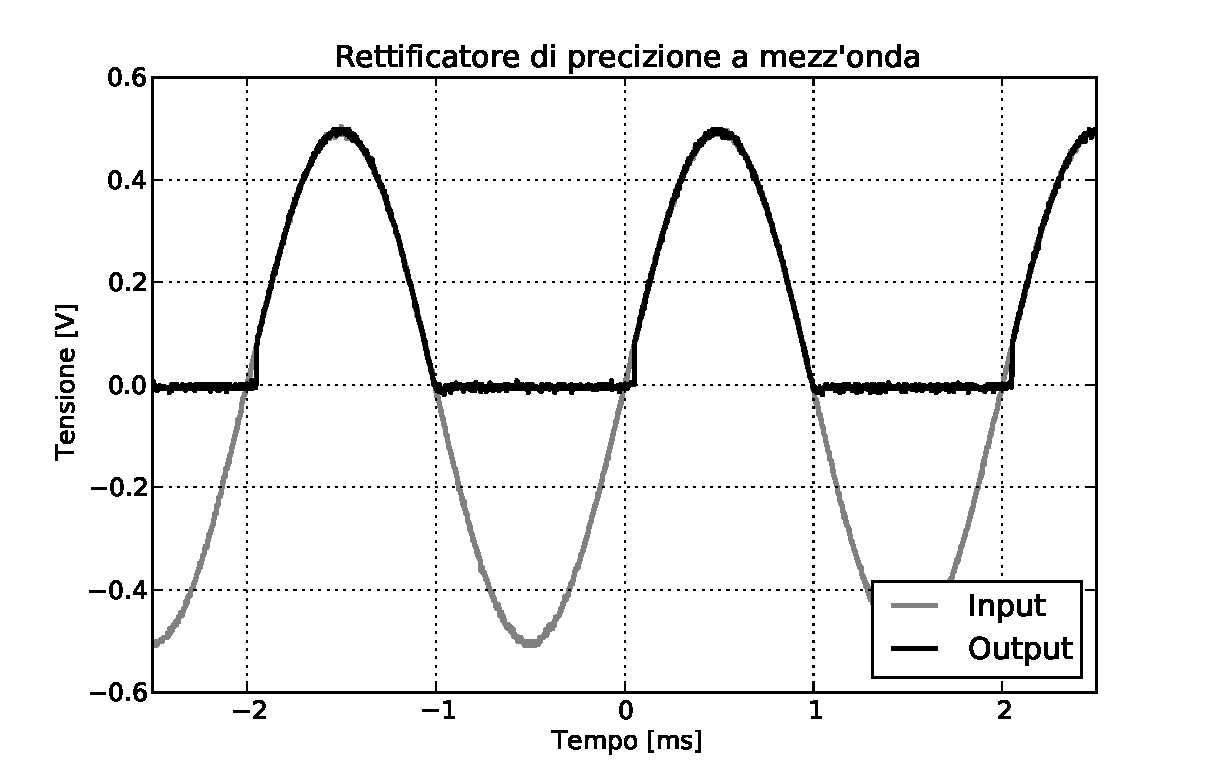
\includegraphics[width=0.7\textwidth]{figure/rett.pdf}
        \caption{Questo grafico illustra l'andamento di $V\ped{out}$, linea nera, in funzione di $V\ped{in}$, linea grigia. Si nota chiaramente, come da previsioni, che la parte negativa del segnale in ingresso impediscse al diodo di condurre, pertanto la tensione di output risulta nulla. Inoltre, come si può osservare, il fronte di salita di $V\ped{out}$ presenta un leggero ritardo rispetto al segnale in ingresso $V\ped{in}$. Questo ritardo è stato stimato essere approssimativamente di circa $(152\pm10)\SI{}{\micro\second}$.}
        \label{fig:radd_plot1}
\end{SCfigure}

\begin{SCfigure}[][p]
        \centering
        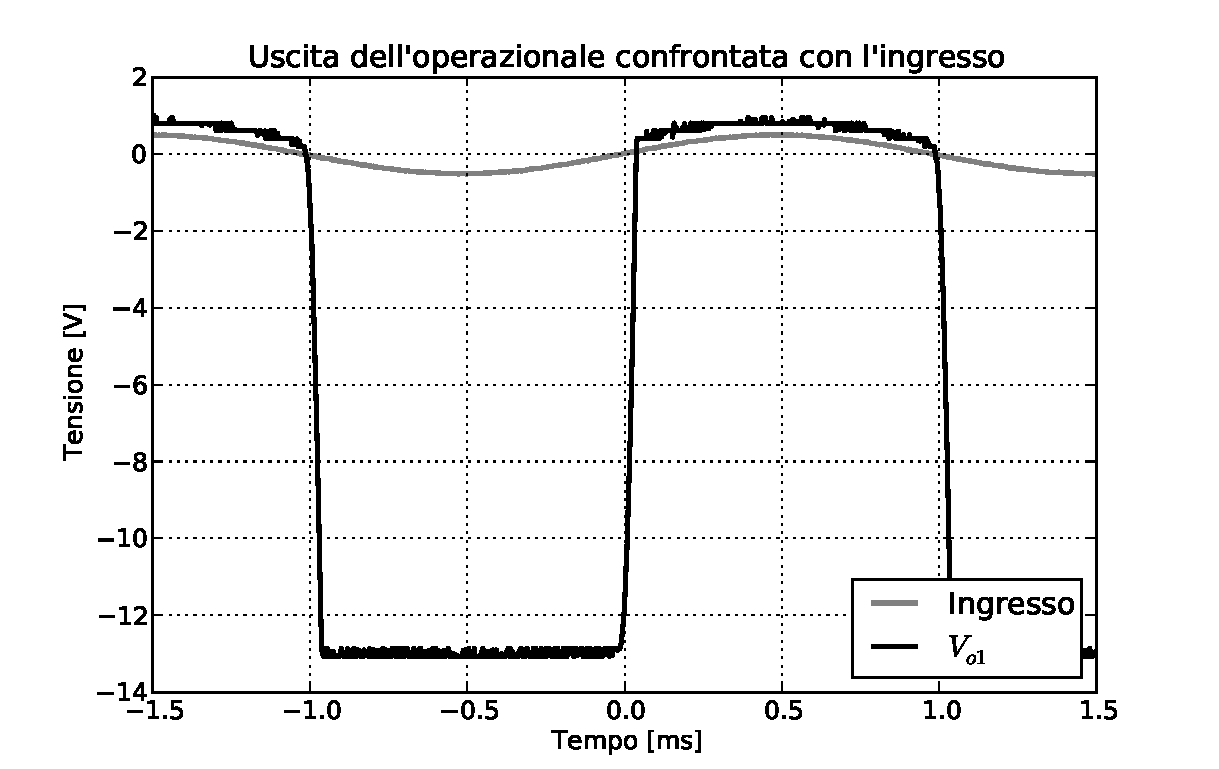
\includegraphics[width=0.7\textwidth]{figure/rett_vo1.pdf}
        \caption{Questo grafico illustra l'andamento di $V\ped{ol}$, linea nera, in funzione di $V\ped{in}$, linea grigia. Si nota chiaramente, come da previsioni, che la parte negativa del segnale in ingresso porta a tensione $V\ped{ol}$ al valore di saturazione negativo $V\ped{sat}^-$. Inoltre è possibile osservare che la differenza di potenziale tra i due segnali, parte positiva, non corrisponde altro che alla caduta in diretta del diodo, che abbiamo stimato essere intorno ai $\SI{0.4}{\volt}$.}
        \label{fig:radd_plot2}
\end{SCfigure}

\begin{SCfigure}[][p]
        \centering
        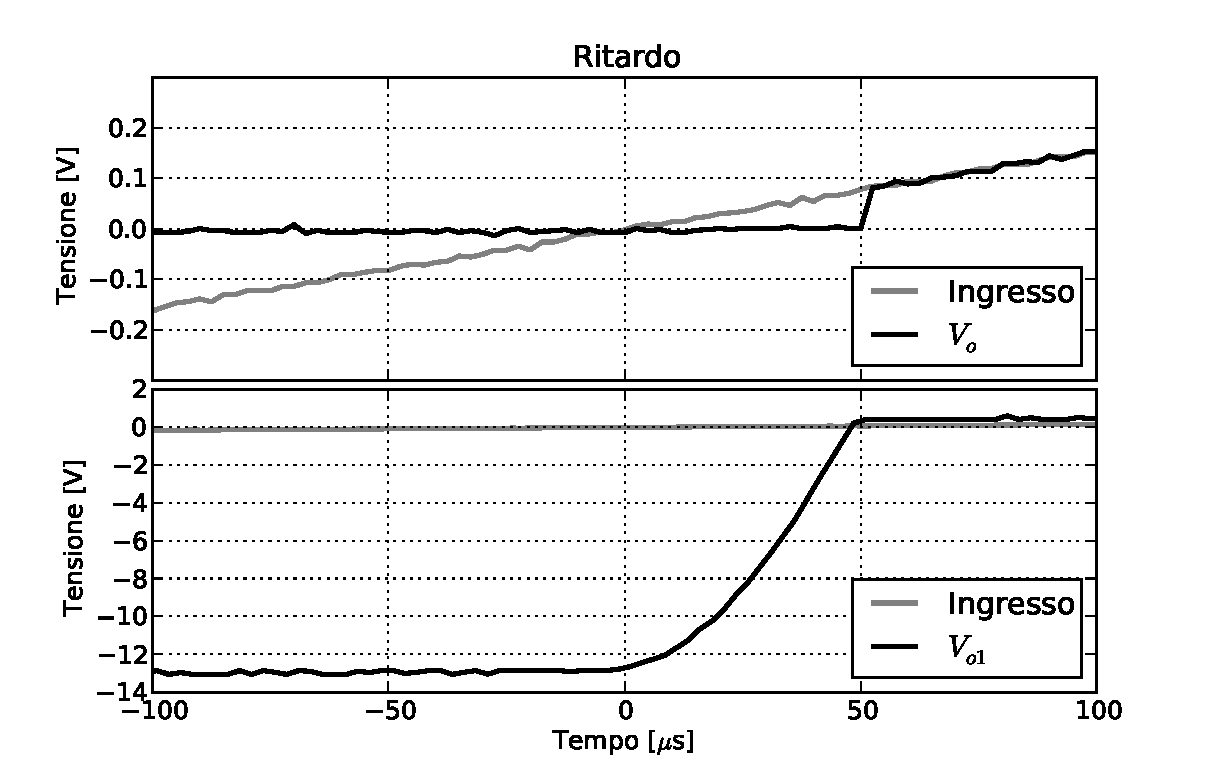
\includegraphics[width=0.7\textwidth]{figure/rett_err.pdf}
        \caption{Questa immagine è un’ingrandimento della zona in cui si presenta il fenomeno del ritardo di $V\ped{out}$ rispetto a $V\ped{in}$ delle precedenti due Figure \ref{fig:radd_plot2} e \ref{fig:radd_plot1}. Il ritardo è circa $\SI{50}{\micro\second}$, e non è possibile giustificarlo con il solo slew rate, limitato, dell’amplificatore operazionale. Nel grafico in basso, la parte iniziale della curva nera (la parte meno pendente) è il momento in cui l’amplificatore operazionale spende tempo ad uscire dalla saturazione negativa.}
        \label{fig:radd_plot3}
\end{SCfigure}

Come è possibile notare dal grafico riportato in Figura \ref{fig:radd_plot3}, vi è un ritardo da parte dell'amplificatore nel seguire, in salita, il segnale in ingresso. Questo ritardo come abbiamo pensato inizialmente non è dovuto allo slew rate dell'amplificatore, anche se in minima parte contribuisce, bensì ad un problema di progettazione del circuito.
Ovvero, nel momento in cui il segnale in ingresso assume valori negativi la tensione $V\ped{ol}$ si trova in saturazione negativa, il diodo è interdetto quindi $V\ped{out}$ che ha lo stesso alore di $V^-$ (causa retroazione negativa), si trova ad una differenza di potenziale nulla. Quindi quando il seganle in ingresso diventa positivo l'amplificatore impiega del tempo prima di portare tutti i suoi componenti interni dalla regione di saturazione negativa ad un regime positivo. Questo lasso di tempo si può identificare pertanto con il ritardo visibile in Figura \ref{fig:radd_plot2}. Inoltre abbiamo notato che aumentando la frequenza del segnale in ingresso il tempo di risposta dell'amplificatore diminuisce. Questo molto probabilmente è dovuto al fatto che sempre meno componenti interni dell'amplifictore si portano completamente in $V\ped{cc}^-$.
Per concludere e dare maggior validità a queste ipotesi possiamo dire che questo ritardo non si accusa quando $V\ped{in}$ passa da positivo a negativo. In questo caso infatti $V\ped{ol}$ può seguire l'andamento del segnale in ingresso in quanto non deve fare fronte ad un improvvisa e importante differenza di potenziale come durante la fase di salita. 
Per oviare a questo problema si possono apportare alcune modifiche al circuto che andremo a discutere nel paragrafo seguente.

\newpage

\subsection*{Raddrizzatore di precisione a semionda ottimizzato}

\begin{wrapfloat}{figure}{O}{0pt}
        \def\svgwidth{0.5\textwidth}
        \subimport{figure/}{radd_ott.pdf_tex}
        \caption{Raddrizzatore di precisione a semionda ottimizzato. Come $V\ped{in}$ è stata fornita un onda sinusoidale con ddp picco picco di $\SI{1.02}{\volt}$ e una frequenza $\nu\,=\,\SI{50}{\hertz}$.}
        \label{fig:radd_ott}
\end{wrapfloat}

In questa sezione ci occupiamo di discutere i vantaggi di un raddrizzatore a semionda realizzato come in Figura \ref{fig:radd_ott}. Come accennato nel paragrafo precedente il grande problema della configurazione precedente è quello che per $V\ped{in}$ negativi $V\ped{ol}$ raggiungeva quasi istantaneamente il valore di tensione tensione $V\ped{cc}^-$ e quindi in salita vi era un lasso temporale in cui $V\ped{out}$ manteneva un valore di tensione nullo a dispetto di un $V\ped{in}$ in ingresso positivo (Figura \ref{radd_plot2}).

Per ovviare a questo inconveniente abbiamo realizzato il circuito illustrato in Figura \ref{fig:radd_ott}. La parte fondamentale risiede nell'inserimento di un secondo diodo ($D_2$) e delle due resistenze $R_1$ e $R_2$.

Passiamo ora ad una discussione sull'andamento del segnale in uscita $V\ped{out}$ in funzione di $V\ped{in}$. Quando $V\ped{in}$ è positivo abbiamo che il segnale di output risulta essere, con le approssimazioni discusse anche nel paragrafo precedente:
\begin{equation}
        \left\{
                \begin{array}{l l l}
                        V\ped{out}\,=\,-V\ped{in}\,\frac{R_2}{R_1}\\
                        \\
                        V\ped{ol}\,=\,-V\ped{in}\,\frac{R_2}{R_1} + \Delta V
                \end{array}
         \right.
         \label{eq:radd_ott}
\end{equation}
pertanto $V\ped{ol}$ è negativo, quindi abbiamo che $D_1$ è in conduzione, mentre $D_2$ è interdetto. Per questi motivi $V\ped{out}$ si troverà a ground, in quanto non vi è passaggio di corrente e sia $R_3$ che $R_2$ sono connesse a ground.

\begin{SCfigure}[][h]
        \centering
        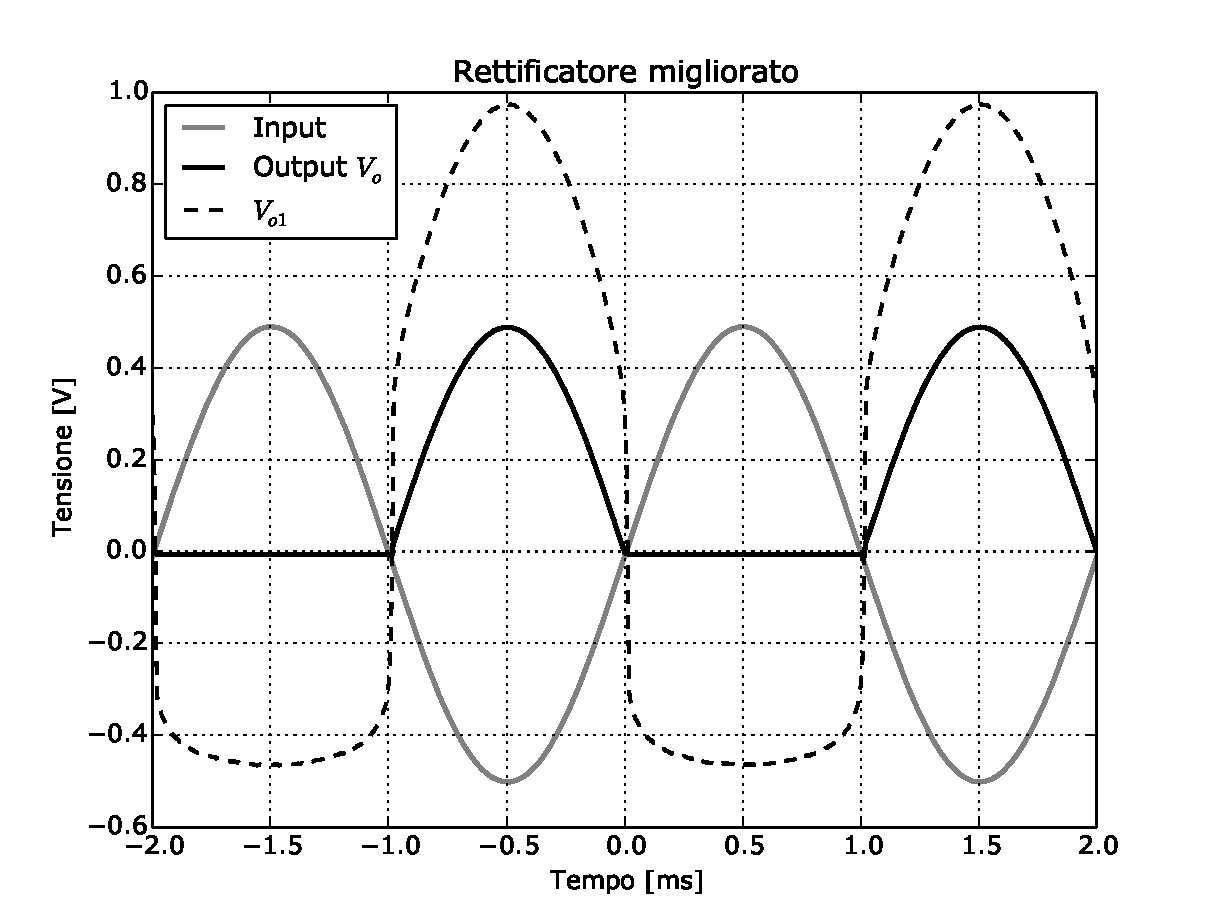
\includegraphics[width=0.7\textwidth]{figure/radd_ott_graph.pdf}
        \caption{Questa immagine raffigura l'andamento delle due diffrenze di potenziale $V\ped{out}$, curva nera, e $V\ped{ol}$, curva tratteggiata, in funzione di $V\ped{in}$. Come è possibile osservare l'andamento di $V\ped{out}$ è molto più pulito rispetto a quanto non fosse per il normale raddrizzatore a semionda. In questo caso non si accusano ritardi significativi, nel fronte in salita, se non quelli dovuti al normale slew-rate dell'amplificatore. Inoltre possiamo notare, che come previsto, la tensione $V\ped{ol}$ non è mai scesa al di sotto dei $\SI{-0.5}{\volt}$.}
        \label{fig:radd_ott_plot}
\end{SCfigure}

Quando $V\ped{in}$ è nullo noi sapiamo che $V^-$ si trova ad un valore di ground virtuale, come anche nel caso in cui $V\ped{in}$ sia positivo o negativo. Quindi $V\ped{out}$ avrà anche esso un valore di tensione nullo. Quindi anche $V\ped{ol}\,=\,\SI{0}{\volt}$ e entrambi i diodi ($D_1$ e $D_2$) risulteranno interdetti e non vi sarà passaggio di corrente.
Nel caso in cui $V\ped{in}$ risulti negativo si ha che il valore di $V\ped{out}$ vale $-V\ped{in}\,\frac{R_2}{R_1}$, che quindi è un valore positivo. In questa configurazione grazie alle equazioni \ref{eq:radd_ott} possimo osservare come $D_1$ sia interdetto, mentre $D_2$ risulti in conduzione e quindi il segnale in uscita $V\ped{out}$ sia la copia di $V\ped{in}$ sfasato di $\pi$. Inoltre possiamo oservare che il minimo valore raggiunto da $V\ped{ol}$ equivale a $\SI{-0.6}{\volt}$ e quindi $V\ped{ol}$ non avrà mai un valore di tensione pari alla saturazione negativa, evitando pertanto il problema osservato nel pargrafo precedente. Ovvero non ci sarà ritardo, durante la fase di salita, da parte dell'amplificatore operazionale nello seguire il segnale in ingresso, dal momento che l'amplificatore non deve commuare da saturazione negativa a valori di tensioni positivi.

Quanto appena detto si può visualizzare facilmente dal grafico riportato in Figura \ref{fig:radd_ott_plot} che descrve l'andamento di $V\ped{out}$ e $V\ped{ol}$ in funzione di $V\ped{in}$.

\subsection*{Amplificatore differenziale}

\begin{wrapfloat}{figure}{O}{0pt}
        \def\svgwidth{0.5\textwidth}
        \subimport{figure/}{diff.pdf_tex}
        \caption{Amplificatore alle differenze usato per annullare gli effetti di rumore ad un segnale in ingresso. Abbiam fornito come sorgente di rumore un segnale sinusoidale di frequenza $\SI{10}{\kilo\hertz}$ e con una ddp. picco picco di $\SI{1}{\volt}$. Il segnale in ingresso, $V\ped{in}$, ha un valore di $\SI{1}{\volt}$ costante.}
        \label{fig:amp_diff}
\end{wrapfloat}

In questo paragrafo vogliamo illustrare la capacità di un circuito con amplificatore alle differenze di annullare il segnale in modo comune, quindi in modo pratico le sorgenti di rumore, e di amplificare solamente il segnale reale.
A tal fine abbiamo realizzato il circuito illustrato in Figura \ref{fig:amp_diff}. Le caratteristiche di questo circuito sono le seguenti: le tensioni di alimentazione positiva e negativa hanno valore di $\pm15\SI{}{\volt}$, il segnale in ingresso ha un valore di $\SI{1}{\volt}$ costante, le resistenze sono state scelte in modo che il guadagno dell'amplificatore differenziale fosse pari a 2. Il rumore è stato simulato con un segnale sinusoidale di frequenza $\SI{10}{\kilo\hertz}$ e con una ddp. picco picco di $\SI{1}{\volt}$.
Infine abbiamo regolato il trimmer affinchè la serie delle due resistenze fosse uguale, dal momento che non ci sono due resistenze perfettamente identiche tra di loro. Questo è stato fatto ponendo  $V\ped{in}\,=\,\SI{0}{\volt}$.

Per questo circuito abbiamo verificato, grazie all'oscilloscopio, che il segnale di output $V\ped{out}$ risultasse costante nel tempo, come $V\ped{in}$, e non presentasse un andamento sinusoidale. Infatti, se tutto funziona correttamente, deve essere la copia amplificata di un fattore 2 di $V\ped{in}$. Possiamo assicurare che da quanto emerso sperimentalmente il circuito ha funzionato correttamente e gli effetti del rumore sul segnale in ingresso sono stati del tutto eliminati. Questa affermazione è corretta fintanto che l'intensità del rumore non raggiunge un valore di circa $\SI{10}{\volt}$pp, nel qual caso il suo contributo al segnale i uscita dall'amplificatore differenziale cominia a non essere trascurabile.

\subsection*{Amplificatore per strumentazione}

\begin{wrapfloat}{figure}{O}{0pt}
        \def\svgwidth{0.5\textwidth}
        \subimport{figure/}{inst_amp.pdf_tex}
        \caption{Amplificatore per strumentazione AD622.}
        \label{fig:inst_amp}
\end{wrapfloat}

Come prima cosa cerciamo di capire cosa sia un'amlificatore per strumentazione.
Un amplificatore da strumentazione (in inglese: Instrumentation amplifier) è un amplificatore operazionale particolarmente adatto per amplificare i segnali provenienti dai trasduttori. Il trasduttore è un qualunque dispositivo che può trasmettere dell'energia da un punto a un altro alterandone alcune delle caratteristiche che la identificano.
Ritornando all'amplificatore per strumentazione: la sua struttura è derivata dall'amplificatore differenziale. Infatti rispetto al classico amplificatore operazionale questo ne presenta due in più che migliorano (aumentandola) l'impedenza d'ingresso e permettono di variare l'amplificazione del segnale differenziale d'ingresso $V\ped{in}$  variando un solo componente: $R_v$. Normalmente si presenta come un unico chip con due pin a cui va connesso il resistore $R_v$.
La relazione che sussiste tra $V\ped{out}$ e il segnale in ingresso è data da:
\begin{equation}
        V\ped{out}\,=\,(-V\ped{in})\,\left(1 + \frac{2R_1}{R_v}\right)\,\frac{R_3}{R_2}
\end{equation}

Detto questo, quello che vogliamo verificare e sperimentare in questo paragrafo è verificare il corretto funzionamento dell'amplificatore per strumentazione misurando la variazione del valore nominale di una resistenza commerciale al variare della temperatura. Proprio per fare questo abbiamo realizzato il circuito riportato in Figura \ref{fig:inst_amp}. Come è possibile notare il circuito presenta in ingresso una configurazione a ponte di Wheatstone. Quindi se nel montaggio del circuito, come è stato fatto, ci preoccupiamo di porre la resistenza $R_s$ lontana dal resto dei componenti possiamo andare a riscaldarla o raffreddarla senza intaccare il corretto funzionamento dei restanti elementi circuitli. Quindi variando la temperatura della resistenza andiamo a variarne il suo stesso valore di resistenza. Infatti vale che: data una resistenza con valore nominale $R$:
\begin{equation}
        \Delta R\,=\,R\,\left(\frac{-200}{10^6}\right) \qquad \text{variazione dal valore nominale di R per variazioni di $^\circ C$.}
        \label{eq:R}
\end{equation}
dove con $\Delta R$ indichiamo la varazione sul valore di resistenza nominale, $-200\,\frac{ppm}{^\circ C}$ è il coefficiente di temperatura.
Quindi quello che andremo a fare è valutare, per variazioni di temperatura operativa di $R_s$ lo sbilanciamento nel ponte di Wheastone. Infatti se alimentiamo il ponte con una tensione $V\ped{in}\,=\,\SI{5}{\volt}$ costante, possiamo misurare direttamente la variazione del segnale in uscita $\Delta V\ped{out}$, infatti:
\begin{equation}
        \Delta V\ped{out}\,=\,G\,V\ped{in}\,\left(\frac{\Delta R_s}{R_s + R\ped{st}}\right)
        \label{eq:V}
\end{equation}
dove con $\Delta R$ indichiamola variazione di $R_s$ dal suo valore nominale, $R\ped{st}$ indichiamo il valore di resistenza $R_s$ alla temperatura operativa $t$. $G$ è il guadagno dellamplificatore per strumentazione che è di circa $G\,\simeq\,1000$.
Quindi con dei semplici passaggi algebrici che conivolgono le equazioni (\ref{eq:R}) e (\ref{eq:V}) possiamo ottenere:
\begin{equation}
        R\ped{st}\,=\,\left(\frac{-200}{10^6}\right)\,G\,\frac{V\ped{out}}{\Delta V}
        \label{eq:R_t}
\end{equation}
Quindi è possibile ricavare il valore di resistenza che assume $R_s$ al variare della tensione $V\ped{out}$, variazione causata dall'alterazione della temperatura di lavoro di $R_s$.

Quello che abbiamo osservato è che a temperatura ambiente $V\ped{out}\,=\,(-1040\pm10)\si{\milli\volt}$, mentre riscaldando la resistenza $R_s$ stringendola con le dita abbiamotrovato un valore dell'output pari a $V\ped{out}\,=\,(-1210\pm10)\si{\milli\volt}$ mentre se raffreddata mediante una bomboletta di refrigerante abbiamo ottenuto che $V\ped{out}\,=\,(-460\pm10)\si{\milli\volt}$. Quindi da questi dati possiamo dedurre che già a temperatura ambiente $R_s$ è minore dell'altra resistenza da $\SI{100}{\ohm}$, quindi se andiamo a riscaldare $R_s$ il suo valore di resistenza diminuisce, mentre se andiamo a raffreddarla aumenta. Tutto questo si può intuire facilmente osservando che la configurazione a ponte di Wheatstone presenta in realtà due partitori di tensione collegati ai due ingressi dell'amplificatore per strumentazione.

\subsection*{Termoresistenza Pt100}

La termoresistenza, comunemente chiamata termometro a resistenza o RTD (dall'inglese Resistance Temperature Detector), è un sensore di temperatura che sfrutta la variazione della resistività di alcuni materiali al variare della temperatura. In particolare per i metalli esiste una relazione lineare che lega resistività e temperatura:
\begin{equation}
    \rho (T)\,=\,\rho_0\cdot[1 + \alpha(T - T_0)]
\end{equation}
dove $T$ è la temperatura, $\rho (T)$ è la resistività del materiale alla temperatura $T$, $\rho_0$ è la resistività del materiale alla temperatura $T_0$ e $\alpha$ un coefficiente che dipende dal materiale.
Sfruttando la relazione che lega resistenza ($R$) e resistività (tramite la sezione $S$ e la lunghezza $L$ del conduttore):
\begin{equation}
    R\,=\,\frac{\rho L}{S} 
\end{equation}
si ottiene:
\begin{equation}
    R(T)\,=\,R_0 \cdot [1 + \alpha(T - T_0)]
\end{equation}
Da quest'ultima relazione si può dunque risalire alla temperatura da una misura di resistenza.

%\begin{wrapfloat}{figure}{O}{0pt}
%        \def\svgwidth{0.5\textwidth}
%        \subimport{figure/}{scopiazzo.png}
%        \caption{Misura di resistenza a 4 fili. In questo paragrafo indicheremo con $R$ quella che nell'immagine è $R\ped{subject}$.}
%        \label{fig:4fili}
%\end{wrapfloat}

Quello che vogliamo fare in questa ultima parte della relazione è effettuare una misura di resistenza di un termosensore PT100 a 4 fili (Figura \ref{fig:4fili}), e grazie al multimetro possiamo conoscere sia il valore di resistenza che di temperatura, quindi non abbiamo bisogno di scomodare nessuna delle equazioni precedenti. Quindi l'obbiettivo è realizzare una simulazione in laboratorio di una condizione di misura equivalente a quella che si avrebbe con dei lunghi cavi di collegamento.
Per questo scopo utilizziamo delle resistenze da $\SI{10}{\ohm}$ in serie sui cavi, in modo da simularne una lunghezza non indifferente e quindi anche una resistenza intrinseca.

Perchè effettuare misure a 4 fili? Il nocciolo della questione è che se effettuassi delle misure a due fili io, nella misura, terrei conto non solo del valore di resistenza del termosensore, ma anche delle resistenze dei cavi, che sono rappresentate dalle due resistenze in serie con questi. Infatti facciamo notare che poiché la resistenza è da soli $100\, \si{\ohm}$ anche una cavo con un impedenza piuttosto piccola, per esempio $1\,\si{\ohm}$ (che potrebbe essere la resistenza di un cavo sottile abbastanza lungo), ci fa compiere un errore dell'$1\%$, cioè di circa $3^\circ$C.
Al contrario grazie alle misure a 4 fili io posso eliminare l’errore della misura causato dalle resistenze dei cavi di connessione. In che modo? Aiutandoci dalla Figura \ref{fig:4fili}, che illustra il circuito realizzato, possimo osservare come: il generatore di corrente costante Itest del multimetro non risente delle resistenze di linea, dal momento che genera una corrente molto elevata che passa sicuramente per $R$. Mentre la misura voltmetrica rileva la diffrenza di ptenziale ai capi di $R$ facendo  scorrere pochissima corrente. Quindi sfruttando le leggi di Ohm e combinando assieme i due strumenti posso risalire al valore esatto della resistenza in esame $R$.

In seguito abbiamo fatto alcune misure di temperatura e abbiamo trovato che: a temperatura ambiente abbiamo misurato $112.00\,\si{\ohm}$ che indica una temperatura di $31^\circ$C. Con la misura a due fili si otteneva invece $134\,\si{\ohm}$ (circa $112 + 2 \times 10$), che significherebbe $78^\circ$C. Riscaldando la resistenza con le dita abbiamo invece letto $114.32\,\si{\ohm}$ ($37^\circ$C), mentre raffreddandola con lo spray abbiamo misurato $89.5\,\si{\ohm}$ ($-27\,^\circ$C).
